\documentclass[a4paper, numbers=withenddot, 11pt]{scrartcl}

\usepackage[utf8]{inputenc}
\usepackage[T1]{fontenc}
\usepackage{lmodern}
\usepackage[ngerman]{babel}
\usepackage[style=alphabetic, backend=biber, bibencoding=utf8]{biblatex}
\addbibresource{literatur.bib}\usepackage{csquotes}
\usepackage{microtype}
\usepackage{graphicx}
\usepackage{amsmath}
\usepackage{setspace}\setstretch{1.1}
\parindent0pt\parskip6pt
\clubpenalty=10000
\widowpenalty=10000
\displaywidowpenalty=10000

\title{{{Titel}}}
\author{{{Autor}}}

\begin{document}
\maketitle

\tableofcontents

\section{Über \LaTeX}

\LaTeX{} is a document preparation system for the \TeX{} typesetting program. It offers programmable desktop publishing features and extensive facilities for automating most aspects of typesetting and desktop publishing, including numbering and  cross-referencing, tables and figures, page layout, bibliographies, and much more. \LaTeX{} was originally written in 1984 by Leslie Lamport and has become the  dominant method for using \TeX; few people write in plain \TeX{} anymore. The current version is \LaTeXe.

\begin{figure}[htbp]
\centerline{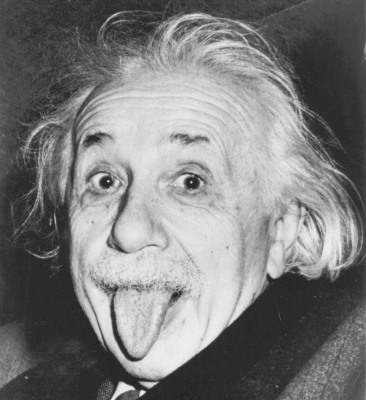
\includegraphics[width=0.3\linewidth]{einstein}}
\caption{Example of a figure caption.}
\label{fig}
\end{figure}

\subsection{Sonstiges}

{{Ergänzender Text }}

Dies ist der Inhalt einer separaten TeX-Datei ...


Zitat aus \cite{scheme} und \cite[17]{knuth}.

\begin{align}
E_0 &= mc^2 \\
E &= \frac{mc^2}{\sqrt{1-\frac{v^2}{c^2}}}
\end{align}

\printbibliography
\end{document}
